% !TEX root=../root.tex

\subsection{Simulation}

\begin{figure}
  \centering
  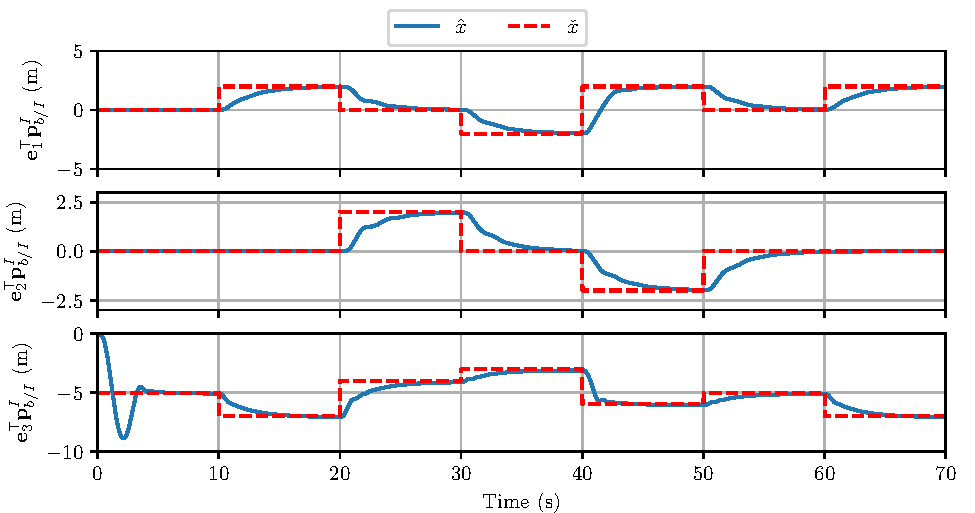
\includegraphics[width=6.5in]{figures/sim_wps_position}
  \caption[LQR Simulation Results Flying Waypoints]{Simulation results for the position of the multirotor UAV given step
  inputs in position. The red dotted line is the desired position and the blue
solid line is the estimated position.}
  \label{f:sim_wps}
\end{figure}

\begin{figure}
  \centering
  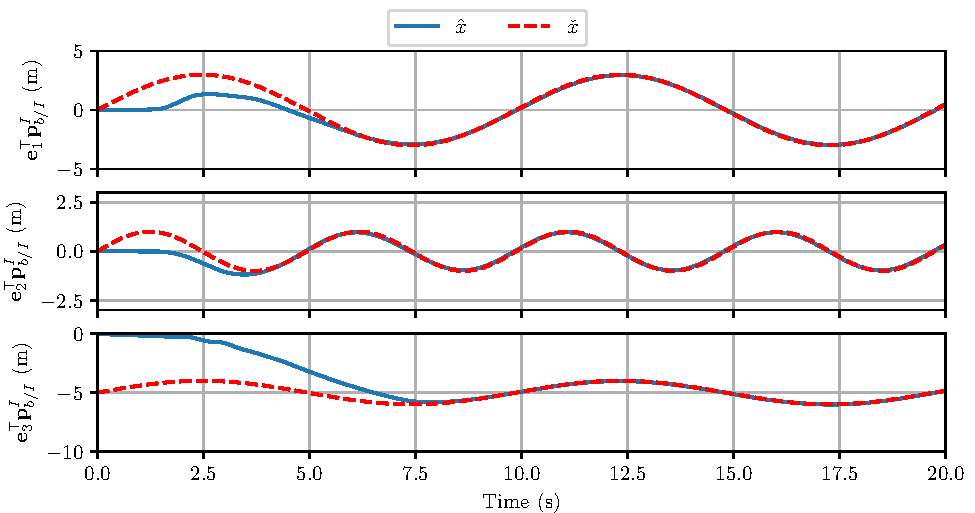
\includegraphics[width=6.5in]{figures/sim_fig8_position}
  \caption[LQR Simulation Results Flying a Trajectory]{Simulation results of a multirotor UAV tracking a figure eight
  trajectory. The red dotted line is the desired position and the blue solid
line is the estimated position.}
  \label{f:sim_fig8}
\end{figure}

Figs.~\ref{f:sim_wps} and~\ref{f:sim_fig8} show simulation results of the
controller following desired position step inputs (waypoints) and a figure-eight trajectory. The
multirotor began the simulations at rest on the ground and converged to the
desired trajectory within a few seconds. In~\figref{f:sim_wps}, we see that the
simulated UAV significantly overshot the initial desired altitude of 5 m, but
relatively smoothly reached the following step inputs. These results are
noteworthy as the desired step inputs caused the error state of the system to be
large, breaking a key assumption of the controller.
% that the error
% state of the system reamins small to be broken.
% break the key assumption of this
% controller, that the 

In~\figref{f:sim_fig8}, we see that the simulated UAV smoothly converged to the
desired trajectory.
After convergence,
% Note that
the figure-eight trajectory
tracking was near perfect even though the feed forward inputs computed
from~\eqref{eq:traj_p}{}--{}~\eqref{eq:traj_omega} did not account for the force due to drag and
the controller did not model thrust dynamics nor torque dynamics.
